% The contents of this file is 
% Copyright (c) 2009-  Charles R. Severance, All Righs Reserved

\chapter{¿Por qué debería aprender a escribir programas?}

Escribir programas (o programar) es una actividad muy
gratificante y creativa. Puedes escribir programas por
muchas razones, desde por mantenerte activo hasta
por resolver un problema difícil de análisis de datos o
por divertirte ayudando a otros a resolver cualquier problema.
Este libro asume que \emph{todo el mundo} necesita saber programar,
y que una vez que sepas programar ya encontrarás tú mismo
la forma de aplicar tus recién adquiridas habilidades.

En nuestra vida diaria estamos rodeados de ordenadores, que van
desde portátiles hasta teléfonos móviles. Podemos pensar en esos
ordenadores como nuestros ``asistentes personales'', que pueden
ocuparse de muchas cosas por nosotros. El hardware en los equipos
que usamos a diario está creado esencialmente para hacernos
continuamente la pregunta,
``¿Qué quieres que haga a continuación?''

\beforefig
\centerline{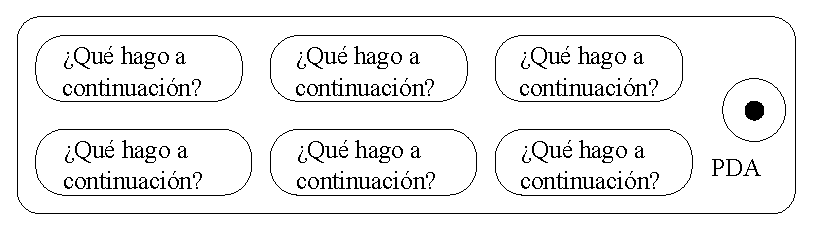
\includegraphics[height=1.00in]{figs2/pda.eps}}
\afterfig

Los programadores añaden un sistema operativo y un conjunto de
aplicaciones al hardware y así tenemos al final un Asistente Personal
Digital que es bastante útil y capaz de ayudarnos a hacer
muchas cosas diferentes.

Nuestros ordenadores son rápidos, tienen gran cantidad de memoria
y podrían resultarnos muy útiles si tan solo conociéramos el idioma
que debemos hablar para explicar al ordenador qué queremos que
´´haga a continuación''. Si conociéramos ese idioma, podríamos pedirle al
ordenador que realizase tareas repetitivas para nosotros. 
Precisamente, el tipo de cosas que los ordenadores hacen mejor
suelen ser el tipo de cosas que los humanos encuentran aburridas
y soporíferas.

Por ejemplo, echa un vistazo a los primeros tres párrafos de este
capítulo y dime cual es la palabra más utilizada y cuántas veces
se ha usado. A pesar de que seas capaz de leer y comprender
las palabras en unos pocos segundos, contarlas es más costoso,
porque no es el tipo de problema que las mentes humanas
fueron diseñadas para resolver. Para un ordenador
es justo al revés: leer y comprender texto
de un trozo de papel es algo complicado para él,
pero contar las palabras y decir cuántas veces
se ha usado la más frecuente es muy sencillo para él:

\beforeverb
\begin{verbatim}
python words.py
Enter file:words.txt
to 16
\end{verbatim}
\afterverb
%
Nuestro ``asistente analista de información personal'' nos dirá
rápidamente que la palabra ``que'' se ha usado ocho veces en los
primeros tres párrafos de este capítulo.

Ese mismo hecho de que los ordenadores sean buenos en cosas
en las que los humanos no lo son es el motivo por el que necesitas
ser capaz de hablar ``idioma de ordenador''. Una vez que hayas
aprendido ese nuevo idioma, podrás delegar tareas mundanas
en tu socio (el ordenador), dejando más tiempo
para ti, para hacer aquellas cosas
en las que estás más capacitado. Serás el encargado
de poner la creatividad, intuición e inventiva a esa
sociedad.

\section{Creatividad y motivación}

Aunque este libro no está dirigido a programadores profesionales, la programación
profesional puede ser un trabajo muy gratificante tanto a nivel financiero como personal.
Construir programas útiles, elegantes e ingeniosos para que otros los usen
es una actividad muy creativa. Tu ordenador o Asistente Personal Digital (APD),
normalmente contienen muchos programas diferentes de multitud de grupos de programadores
distintos, cada uno de los cuales compite por tu atención e interés.
Ellos intentan hacer lo mejor que saben para adaptarse a tus necesidades y proporcionarte
una buena experiencia de usuario en el proceso. En algunos casos, cuando eliges un programa
determinado, los programadores son directamente recompensados por tu elección.

Si pensamos en los programas como salida creativa para grupos de programadores,
tal vez la siguiente figura sea una versión más acertada de tu APD:

\beforefig
\centerline{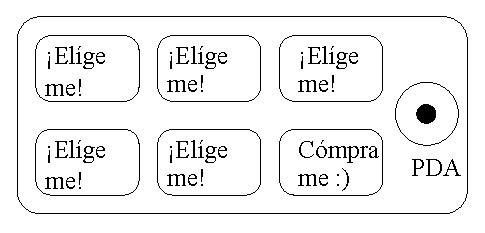
\includegraphics[height=1.00in]{figs2/pda2.eps}}
\afterfig

Por ahora, nuestra motivación principal no es conseguir dinero o gustar más a los usuarios
finales, sino ser más productivos para nosotros mismos en el manejo de los datos e
información que encontraremos en nuestras vidas.
Al principio, serás tanto programador como usuario final de tus propios programas.
Cuando ganes en habilidad como programador y la programación se haga más creativa para ti,
tus ideas podrán avanzar desarrollando programas para otros.

\section{Arquitectura hardware del ordenador}
\index{hardware}
\index{hardware!architecture}

Antes de que empecemos a aprender el idioma que deberemos hablar
para dar instrucciones a los ordenadores o desarrollar
software, necesitamos aprender un poco acerca de cómo
están construidos los ordenadores. Si desmontaras
tu ordenador o teléfono móvil y mirases dentro,
encontrarías los siguientes componentes:

\beforefig
\centerline{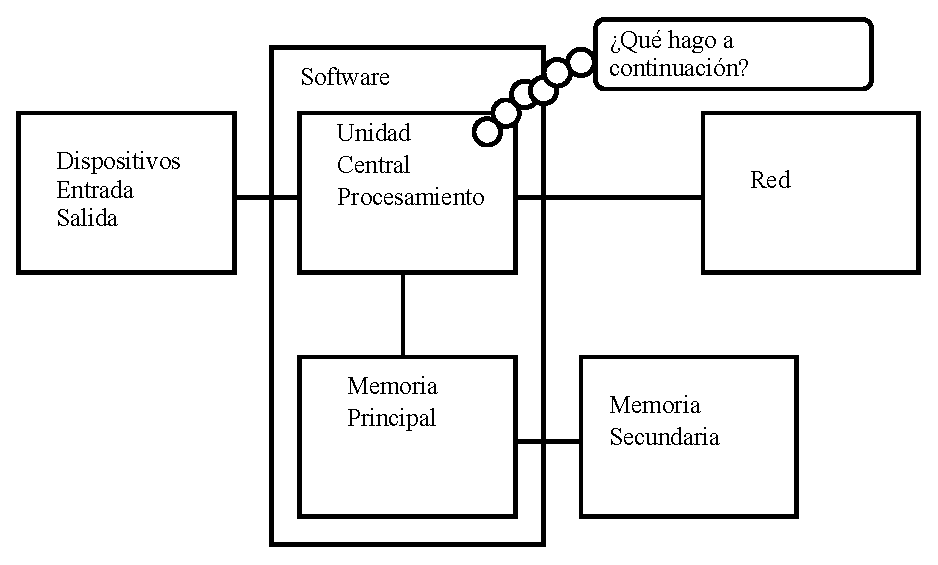
\includegraphics[height=2.50in]{figs2/arch.eps}}
\afterfig

Las definiciones de alto-nivel de estos componentes son las siguientes:

\begin{itemize}

\item La {\bf Unidad Central de Procesamiento} (o CPU) es
la parte del ordenador que está construida para estar obsesionada
con el ``¿qué es lo siguiente?'' Si tu ordenador está clasificado
como de 3.0 Gigahercios, significa que la CPU va a preguntar ``¿Qué hago a continuación?''
tres mil millones de veces por segundo. Tendrás que aprender a hablarle muy
rápido para mantener el ritmo de tu CPU.

\item La {\bf Memoria Principal} se usa para almacenar la información
que la CPU necesita enseguida. La memoria principal es casi
tan rápida como la CPU. Pero la información almacenada en la memoria
principal se desvanece cuando el ordenador se apaga.

\item La {\bf Memoria Secundaria} Es también utilizada para almacenar
información, pero es mucho más lenta que la memoria principal.
La ventaja de la memoria secundaria es que puede mantener
almacenada la información incluso cuando el ordenador está apagado.
Ejemplos de memoria secundaria son las unidades de disco o las
memorias flash (que se encuentran normalmente en lápices USB y
reproductores de música portátiles).

\item Los {\bf Dispositivos de Entrada y Salida} son simplemente
la pantalla, teclado, ratón, micrófono, altavoces, touchpad, etc.
Son todos los aparatos que utilizamos para interactuar con el ordenador.

\item En la actualidad, la mayoría de los ordenadores disponen también de una
{\bf Conexión de Red} para recibir información a través de la red.
Podemos pensar en la red como en un sitio muy lento donde se almacenan
y recuperan datos que puede no estar siempre ``lista''. Así que en cierto sentido,
la red es una forma lenta y a veces poco fiable de
{\bf Memoria Secundaria}.

\end{itemize}

Aunque la mayoría de los detalles de cómo funcionan estos componentes es mejor
dejarlos para los que construyen ordenadores, resulta útil tener cierta terminología
con la que referirnos a estas distintas partes mientras escribimos nuestros programas.

Como programador, tu trabajo es usar y orquestar cada uno de esos
recursos para resolver el problema que necesites solucionar
y analizar los datos que obtengas de la solución. Como programador, principalmente
estarás ``hablando'' con la CPU y diciéndole qué debe hacer a continuación.
A veces le dirás a la CPU que use la memoria principal,
la memoria secundaria o los dispositivos de entrada/salida.

\beforefig
\centerline{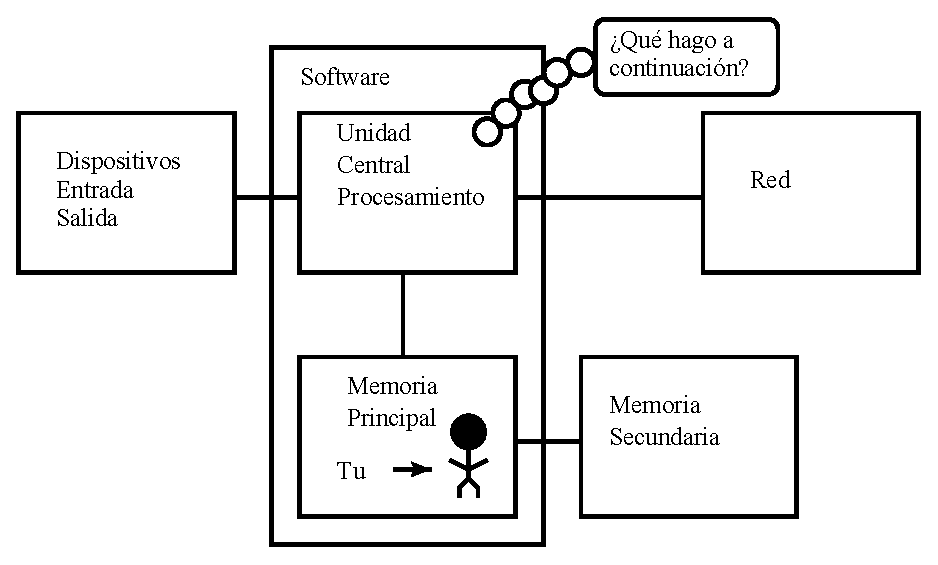
\includegraphics[height=2.50in]{figs2/arch2.eps}}
\afterfig

Tú debes ser la persona que conteste a la pregunta de la CPU ``¿Qué hago a continuación?''.
Pero sería muy incómodo encogerse hasta los 5mm de altura
y meterse dentro del ordenador sólo para poder pasarle un comando
tres mil millones de veces por segundo. Así que en vez de eso,
deberás ponerle por escrito las instrucciones por adelantado.
Llamaremos a esas instrucciones almacenadas un {\bf programa}, y al acto
de escribir esas instrucciones y conseguir que
sean correctas, {\bf programar}.

\section{Comprendiendo la programación}

Durante el resto de este libro, intentaremos convertirte en una persona
hábil en el arte de programar. Al final serás un
{\bf programador} --- tal vez no un programador profesional, pero
al menos tendrás la capacidad de echar un vistazo a un problema de análisis
de datos/información y desarrollar un programa para resolverlo.

\index{problem solving}

En cierto sentido, necesitas dos habilidades para ser un programador:

\begin{itemize}

\item En primer lugar, debes dominar el lenguaje de programación (Python) -
debes conocer su vocabulario y su gramática. Debes ser capaz de escribir
las palabras en este nuevo lenguaje correctamente y saber cómo construir
``frases'' bien formadas en este lenguaje.

\item En segundo lugar, debes ``contar una historia''. Al escribir una historia,
combinas palabras y frases para transmitir una idea al lector.
Son necesarios habilidad y arte para construir la historia, y esa habilidad
se mejora precisamente escribiendo y teniendo cierta retroalimentación.
En programación, nuestro programa es la ``historia'' y el problema
que estás tratando de resolver es la ``idea''.

\end{itemize}

Una vez que aprendas un lenguaje de programación como Python, encontrarás
mucho más sencillo aprender un segundo lenguaje como JavaScript o C++.
Cada nuevo lenguaje de programación tendrá un vocabulario y gramática muy
diferentes, pero la forma de resolver problemas
va a ser la misma en todos ellos.

Aprenderás el ``vocabulario'' y ``frases'' de Python muy rápidamente.
Te constará un poco más ser capaz de escribir un programa coherente
para resolver un problema nuevo. Se enseña a programar de forma muy similar
a como se enseña a escribir. Se comienza leyendo y explicando programas,
después se escriben programas simples, y se va incrementando la complejidad
de ellos poco a poco. En algún momento ``encuentras tu musa'' y comienzas
a descubrir los patrones por ti mismo, de modo que eres capaz de tomar un
problema y escribir un programa para resolverlo. Y una vez has llegado a ese
punto, la programación se convierte en un proceso muy agradable y creativo.

Comenzaremos con el vocabulario y estructura de los programas en Python. Ten
paciencia si la simplicidad de los ejemplos te recuerdan a cuando empezaste
a leer por primera vez.

\section{Palabras y frases}
\index{programming language}
\index{language!programming}

A diferencia de los idiomas humanos, el vocabulario de Python es actualmente
bastante reducido. Llamamos a ese ``vocabulario'' las ``palabras reservadas''.
Son palabras que tienen un significado muy especial para Python. Cuando Python
encuentra esas palabras en un programa, tienen un significado y sólo uno para Python.
Más adelante, cuando escribas programas, compondrás tus propias palabras, que tendrán significado para ti, llamadas {\bf variables}. Tendrás una gran libertad para escoger los nombres para tus variables, pero no podrás usar ninguna de las palabras reservadas de Python.

Cuando se entrena a un perro, se usan palabras especiales como
``siéntate'', ``quieto'', y ``traelo''. Cuando hablas con un perro y
no usas ninguna de las palabras reservadas, sólo consigues que te mire
con cara extraña hasta que le digas una palabra reservada.
Por ejemplo, si le dices:
``Me gustaría que hubiera más gente que se dedicase a caminar para mejorar su salud'',
lo que la mayoría de los perros oirían sería:
``bla bla bla {\bf caminar} bla bla bla bla.''.
Esto se debe a que ``caminar'' es una palabra reservada en el idioma del perro.
Mucha gente podría indicar que le idioma entre humanos y gatos no tiene
palabras reservadas\footnote{\url{http://xkcd.com/231/}}.

Las palabras reservadas en el idioma en que los humanos hablan con
Python incluye las siguientes:

\beforeverb
\begin{verbatim}
and       del       from      not       while    
as        elif      global    or        with     
assert    else      if        pass      yield    
break     except    import    print              
class     exec      in        raise              
continue  finally   is        return             
def       for       lambda    try
\end{verbatim}
\afterverb
%
Eso es todo, y a diferencia de un perro, Python ya está completamente entrenado.
Cuando dices ``try'', Python lo intentará cada vez que se lo digas sin
equivocarse.\footnote{``try'' en inglés puede traducirse como ``inténtalo''(N. del Trad.)}

Aprenderemos esas palabras reservadas y cómo usarlas a su debido tiempo,
pero por ahora nos centraremos en la equivalencia en Python de ``habla''
(en el idioma humano-a-perro). Lo bueno de pedirle a Python que hable
es que podemos incluso decirle qué debe decir, pasándole un mensaje entre comillas:

\beforeverb
\begin{verbatim}
print '¡Hola, mundo!'
\end{verbatim}
\afterverb

Y ya hemos escrito nuestra primera frase sintácticamente correcta en Python.
Nuestra sentencia comienza con la palabra reservada {\bf print}, seguida
por una cadena de texto de nuestra elección, encerrada entre comillas simples.

\section{Conversando con Python}

Ahora que ya conocemos una palabra y una sentencia simple en Python,
debemos aprender cómo comenzar una conversación con Python para probar
nuestras nuevas habilidades.

Antes de que puedas conversar con Python, debes en primer lugar instalar
el software de Python en tu ordenador, y aprender a ponerlo en marcha.
La explicación sobre cómo conseguirlo excede el propósito de este capítulo,
así que te sugiero consultar \url{www.pythonlearn.com}, donde tengo
instrucciones detalladas y capturas de pantallas sobre cómo instalar y poner en marcha
Python en sistemas Macinstosh y Windows. En algún momento, terminarás en un terminal
o ventana de comandos, escribirás {\bf python}, y el intérprete de Pyhton
comenzará a ejecutarse en modo interactivo, apareciendo algo como lo siguiente:

\index{interactive mode}

\beforeverb
\begin{verbatim}
Python 2.6.1 (r261:67515, Jun 24 2010, 21:47:49) 
[GCC 4.2.1 (Apple Inc. build 5646)] on darwin
Type "help", "copyright", "credits" or "license" for more information.
>>> 
\end{verbatim}
\afterverb
%
El indicador {\tt >>>} es el modo que tiene el intérprete de Python de preguntarte:
``¿Qué quieres que haga a continuación?''. Python está preparado para tener una conversación contigo. Todo lo que tienes que hacer es hablar el idioma de Python.

Imaginemos por ejemplo que no conoces ni siquiera la más simple de las palabras o frases del lenguaje Python. Tal vez quiera usar la línea habitual que los astronautas usan cuando aterrizan en un planeta remoto y quieren hablar con sus habitantes:

\beforeverb
\begin{verbatim}
>>> Venimos en son de paz, por favor llevadnos ante vuestro lider
  File "<stdin>", line 1
    Venimos en son de paz, por favor llevadnos ante vuestro lider
         ^
SyntaxError: invalid syntax
>>> 
\end{verbatim}
\afterverb
%
Esto no está funcionando. A menos que pienses en algo rápido,
los habitantes del planeta probablemente te clavarán sus lanzas,
te ensartarán en un asador, te cocinarán sobre el fuego, y te usarán como cena.

Por suerte has comprado una copia de este libro durante el viaje, así que lo hojeas
hasta llegar precisamente a esta página y pruebas de nuevo:

\beforeverb
\begin{verbatim}
>>> print '¡Hola, mundo!'
¡Hola, mundo!
\end{verbatim}
\afterverb
%
Esto tiene mejor aspecto, así que intentas comunicarte un poco
más:

\beforeverb
\begin{verbatim}
>>> print 'Tú debes ser el dios legendario que viene del cielo'
Tú debes ser el dios legendario que viene del cielo
>>> print 'Hemos estado esperándote durante mucho tiempo'
Hemos estado esperándote durante mucho tiempo
>>> print 'Nuestras leyendas dicen que debes estar muy sabroso con mostaza'
Nuestras leyendas dicen que debes estar muy sabroso con mostaza
>>> print 'Vamos a tener un festín esta noche a menos que digas
  File "<stdin>", line 1
    print 'Vamos a tener un festín esta noche a menos que digas
                                                              ^
SyntaxError: EOL while scanning string literal
>>> 
\end{verbatim}
\afterverb
%
La conversación fue bien durante un rato, y entonces, en cuanto
cometiste un pequeño error usando el lenguaje Python, Python
volvió a apuntarte con las lanzas.

En este momento, ya deberías haberte dado cuenta de que, a pesar de que Python
es increíblemente complejo, potente y muy exigente con
la sintaxis que debes usar para comunicarte con él, Python {\em no} es
inteligente. En realidad tan sólo estás teniendo una conversación
contigo mismo, eso sí, usando una sintaxis correcta.

En cierto sentido, cuando usas un programa escrito por otra persona,
la conversación se mantiene entre ti y esos otros programadores,
con Python actuando como intermediario. Python es un
modo de que los creadores de programas puedan expresar cómo creen
que deben desarrollarse las conversaciones. Y dentro
de unos pocos capítulos más, tú serás uno de esos programadores
que usan Python para hablar con los usuarios de tus programas.

Antes de teminar nuestra primera conversación con el intérprete
de Python, probablemente debas saber cual es el modo correcto
de decir ``adios'' cuando estás interactuando con los
habitantes del Planeta Python:

\beforeverb
\begin{verbatim}
>>> adios
Traceback (most recent call last):
  File "<stdin>", line 1, in <module>
NameError: name 'adios' is not defined

>>> if you don't mind, I need to leave
  File "<stdin>", line 1
    if you don't mind, I need to leave
             ^
SyntaxError: invalid syntax

>>> quit()
\end{verbatim}
\afterverb
%
Te habrás dado cuenta de que el error es diferente en los primeros
dos intentos incorrectos. El segundo error es diferente porque
{\bf if} es una palabra reservada, y Python encuentra la palabra
reservada y cree que estás intentando decirle algo, pero encuentra
la sintaxis de la sentencia incorrecta.

El modo correcto de decir ``adios'' a Python es introducir
{\bf quit()} en el indicador interactivo {\tt >>>}.
Probablemente te hubiera llevado un buen rato adivinarlo,
así que es posible que tener un libro a mano
esté empezando a resultarte útil.

\section{Terminología: intérprete y compilador}

Python es un lenguaje de {\bf alto nivel}, que intenta ser relativamente
sencillo de escribir y leer para los humanos y de leer y procesar para
los ordenadores. Hay otros lenguajes de alto nivel, como Java, C++,
PHP, Ruby, Basic, Perl, JavaScript, y muchos más. El hardware que está
actualmente dentro del la Unidad Central de Procesamiento (CPU) no comprende
ninguno de estos lenguajes de alto nivel.

La CPU comprende un lenguaje que se llama {\bf código máquina}. El código
máquina es muy simple y francamente muy cansado de escribir, porque
en él todo está representado por ceros y unos:

\beforeverb
\begin{verbatim}
01010001110100100101010000001111
11100110000011101010010101101101
...
\end{verbatim}
\afterverb
%
El código máquina superficialmente parece muy sencillo, dado que sólo hay
ceros y unos, pero su sintaxis es incluso más complicada
y mucho más intrincada que Python. Así que muy pocos programadores
usan este lenguaje. En vez de eso, se han construído varios traductores para
permitir a los programadores escribir en lenguajes de alto nivel, como Python
o JavaScript, y esos traductores convierten luego los programas a código máquina
para que la CPU pueda ejecutarlos.

Dado que el código máquina está ligado al hardware del ordenador, ese código
no es {\bf portable} a través de diferentes tipos de hardware. Los programas escritos
en lenguajes de alto nivel pueden ser trasladados entre ordenadores diferentes usando
un intérprete diferente en la nueva máquina o recompilando el código para crear
una versión en código máquina del programa para el nuevo equipo.

Estos traductores de lenguajes de programación se clasifican en dos categorías generales:
(1) intérpretes y (2) compiladores.

Un {\bf intérprete} lee el código fuente del programa tal y como lo ha escrito
el programador, analiza el código fuente e interpreta las instrucciones al vuelo.
Python es un intérprete y cuando estamos haciéndolo funcionar de forma interactiva,
podemos escribir una línea de Python (una sentencia), y Python la procesa inmediatamente
y queda listo para que podemos escribir otra nueva línea.

Algunas de las líneas de Python le indican que lo que queremos es recordar cierto
valor para más tarde. Debemos elegir un nombre para que ese valor sea recordado y
podremos usar ese nombre simbólico para recuperar el valor más tarde. Usamos el
término {\bf variable} para referirnos a las etiquetas que utilizamos para manejar esos
datos almacenados.

\beforeverb
\begin{verbatim}
>>> x = 6
>>> print x
6
>>> y = x * 7
>>> print y
42
>>> 
\end{verbatim}
\afterverb
%
En este ejemplo, le pedimos a Python que recuerde el valor seis y use la etiqueta {\bf x},
para que podemos recuperar ese valor más tarde. Comprobamos que Python ha guardado de
momento el valor usando {\bf print}. A continuación le pedimos a Python que recupere {\bf x}, lo multiplique por siete y coloque el nuevo valor calculado en {\bf y}. Finalmente, le pedimos a Python que imprima el valor que está actualmente en {\bf y}.

Aunque estemos escribiendo estos comandos en Python línea por línea, Python
los está tratando como una secuencia ordenada de declaraciones, de modo
que las últimas declaraciones son capaces de recuperar datos creados en las
anteriores. Estamos escribiendo nuestro primer párrafo simple con cuatro frases
en un orden lógico y útil.

La naturaleza de un {\bf intérprete} es ser capaz de tener una conversación interactiva como se muestra más arriba. Un {\bf compilador} necesita que le entreguen el programa
completo en un archivo, y después
ejecuta un proceso para trasladar el código fuente de alto nivel a código máquina.
A continuación el compilador guarda el código máquina resultante en un archivo para su
posterior ejecucación. 

Si usas un sistema Windows, a menudo esos programas ejecutables en código máquina tienen un sufijo como ``.exe'' or ``.dll'', que indican ``executable (ejecutable)'' y ``dynamic
link library (librería de enlace dinámico)'' respectivamente. En Linux y Macinstosh
no hay un sufijo que marque de forma única un archivo como ejecutable.

Si abrieras un archivo ejecutable en un editor de texto, se mostraría algo
completamente disparatado e ilegible:

\beforeverb
\begin{verbatim}
^?ELF^A^A^A^@^@^@^@^@^@^@^@^@^B^@^C^@^A^@^@^@\xa0\x82
^D^H4^@^@^@\x90^]^@^@^@^@^@^@4^@ ^@^G^@(^@$^@!^@^F^@
^@^@4^@^@^@4\x80^D^H4\x80^D^H\xe0^@^@^@\xe0^@^@^@^E
^@^@^@^D^@^@^@^C^@^@^@^T^A^@^@^T\x81^D^H^T\x81^D^H^S
^@^@^@^S^@^@^@^D^@^@^@^A^@^@^@^A\^D^HQVhT\x83^D^H\xe8
....
\end{verbatim}
\afterverb
%
No es fácil leer o escribir código máquina, así que está bien que tengamos
{\bf intérpretes} y {\bf compiladores} que nos permitan escribir en lenguajes
de alto nivel, como Python o C.

En este momento de la discusión acerca de compiladores e intérpretes, deberías
estar preguntándote algunas cosas sobre el mismo intérprete de Python. ¿En qué
lenguaje ha sido escrito? ¿Ha sido escrito en un lenguaje compilado? Cuando escribimos ``python'', ¿qué es exactamente lo que ocurre?

El intérprete de Python está escrito en un lenguaje de alto nivel llamado ``C''.
Puedes ver el código fuente actual del intérprete de Python acudiendo a
\url{www.python.org}, y trabajar como quieras con su código fuente.
Así que Python es él mismo también un programa, y está compilado en código máquina.
Cuando instalaste Python en tu ordenador (o el vendedor lo instaló),
pusiste una copia del código máquina del programa Python traducido para tu sistema.
En Windows, el ejecutable en código máquina del propio Python es probablemente
un archivo con un nombre como:

\beforeverb
\begin{verbatim}
C:\Python27\python.exe
\end{verbatim}
\afterverb
%
Esto ya es más de lo que en realidad necesitas saber para ser un programador en Python,
pero a veces es mejor responder a estas típicas preguntillas justo
al principio.

\section{Escribiendo un programa}

Escribir frases en el intérprete de Python es un buen modo de experimentar
con las características de Python, pero no se recomienda para resolver problemas
más complejos.

Cuando queremos escribir un programa,
usamos un editor de texto para escribir las instrucciones de Python en un archivo,
que se denomina un {\bf script}. Por
convención, los scripts en Python tienen nombres que terminan en {\tt .py}.

\index{script}

Para ejecutar un script, tienes que indicarle al intérprete de Python
el nombre del archivo. En una ventana de comandos de Unix o Windows,
puedes escribir {\tt python hello.py} así:

\beforeverb
\begin{verbatim}
csev$ cat hello.py
print '¡Hola, mundo!'
csev$ python hello.py
¡Hola, mundo!
csev$
\end{verbatim}
\afterverb
%
El ``csev\$'' es el indicador del sistema operativo, y el ``cat hello.py'' nos
está mostrando que el archivo ``hello.py'' contiene un programa Python de una línea
que imprime una cadena.

Estamos llamando al intérprete de Pyhton e indicándole que lea el código fuente del
archivo ``hello.py'', en vez de ir escribiendo nosotros las líneas de código Python
de forma interactiva.

Habrás notado que no es necesario poner {\\bf quit()} al final del programa
Python en el archivo. Cuando Python está leyendo tu código fuente
desde un archivo, sabe parar cuando llega al final del fichero.

\section{¿Qué es un programa?}

La definición más básica de un {\bf programa} es que se trata de una
secuencia de sentencias de Python que han sido creadas para hacer algo.
Incluso nuestro simple script {\bf hello.py} es un programa. Es un programa
de una sola línea y no particularmente útil, pero en su más estricta definición,
es un programa Python. 

Debería ser más sencillo comprender qué es un programa si pensamos en un problema
que pudiera resolverse creando un programa, y a continuación observar cómo sería programa
que resolvería ese problema.

Imaginemos que estás haciendo una investigación sobre Cómputo Social en los mensajes
de Facebook, y estás interesado en saber cuál es la palabra que se usa con mayor frecuencia
en una serie de mensajes. Podrías imprimir la cadena de mensajes de Facebook y estudiar
detenidamente el texto, buscando la palabra más común, pero eso te llevaría mucho tiempo
y sería muy probable que cometieses errores. Sería más inteligente escribir un programa
en Python para realizar la tarea rápidamente y con precisión, y así podrías emplear el fin
de semana en hacer algo divertido.

Por ejemplo, mira el texto siguiente acerca de un payaso y un coche. Mira al
texto y busca cual es la palabra más común y cuántas veces se repite.

\beforeverb
\begin{verbatim}
el payaso corrió detrás del coche y el coche se metió en la carpa
y la carpa se cayó sobre el payaso y el coche
\end{verbatim}
\afterverb
%
Después imagina que estás haciendo esta tarea buscando en millones de líneas de
texto. Francamente, te resultaría más rápido aprender Python y escribir un
programa para contar las palabras que revisar manualmente todas las palabras.

La buena noticia es que a mí ya se me ha ocurrido un programa
simple para encontrar la palabra más común en un archivo de texto. Lo he escrito,
probado, y ahora te lo doy a ti para que lo uses y puedas ahorrarte algo de tiempo.

\beforeverb
\begin{verbatim}
name = raw_input('Introduce archivo:')
handle = open(name, 'r')
text = handle.read()
words = text.split()
counts = dict()

for word in words:
   counts[word] = counts.get(word,0) + 1

bigcount = None
bigword = None
for word,count in counts.items():
    if bigcount is None or count > bigcount:
        bigword = word
        bigcount = count

print bigword, bigcount
\end{verbatim}
\afterverb
%
You don't even need to know Python to use this program.  You will need to get through 
Chapter 10 of this book to fully understand the awesome Python techniques that were
used to make the program.  You are the end user, you simply use the program and marvel
at its cleverness and how it saved you so much manual effort.
You simply type the code 
into a file called {\bf words.py} and run it or you download the source 
code from \url{http://www.pythonlearn.com/code/} and run it.

\index{program}
This is a good example of how Python and the Python language are acting as an intermediary
between you (the end user) and me (the programmer).  Python is a way for us to exchange useful
instruction sequences (i.e., programs) in a common language that can be used by anyone who 
installs Python on their computer.  So neither of us are talking {\em to Python},
instead we are communicating with each other {\em through} Python.

\section{The building blocks of programs}

In the next few chapters, we will learn more about the vocabulary, sentence structure,
paragraph structure, and story structure of Python.  We will learn about the powerful
capabilities of Python and how to compose those capabilities together to create useful
programs.

There are some low-level conceptual patterns that we use to construct programs.  These
constructs are not just for Python programs, they are part of every programming language
from machine language up to the high-level languages.

\begin{description}

\item[input:] Get data from the ``outside world''.  This might be 
reading data from a file, or even some kind of sensor like 
a microphone or GPS.  In our initial programs, our input will come from the user
typing data on the keyboard.

\item[output:] Display the results of the program on a screen
or store them in a file or perhaps write them to a device like a
speaker to play music or speak text.

\item[sequential execution:] Perform statements one after
another in the order they are encountered in the script.

\item[conditional execution:] Check for certain conditions and
then execute or skip a sequence of statements.

\item[repeated execution:] Perform some set of statements 
repeatedly, usually with
some variation.

\item[reuse:] Write a set of instructions once and give them a name
and then reuse those instructions as needed throughout your program.

\end{description}

It sounds almost too simple to be true, and of course it is never
so simple.  It is like saying that walking is simply
``putting one foot in front of the other''.  The ``art'' 
of writing a program is composing and weaving these
basic elements together many times over to produce something
that is useful to its users.

The word counting program above directly uses all of 
these patterns except for one.

\section{What could possibly go wrong?}

As we saw in our earliest conversations with Python, we must
communicate very precisely when we write Python code.  The smallest
deviation or mistake will cause Python to give up looking at your
program.

Beginning programmers often take the fact that Python leaves no
room for errors as evidence that Python is mean, hateful, and cruel.
While Python seems to like everyone else, Python knows them 
personally and holds a grudge against them.  Because of this grudge,
Python takes our perfectly written programs and rejects them as 
``unfit'' just to torment us.

\beforeverb
\begin{verbatim}
>>> primt 'Hello world!'
  File "<stdin>", line 1
    primt 'Hello world!'
                       ^
SyntaxError: invalid syntax
>>> primt 'Hello world'
  File "<stdin>", line 1
    primt 'Hello world'
                      ^
SyntaxError: invalid syntax
>>> I hate you Python!
  File "<stdin>", line 1
    I hate you Python!
         ^
SyntaxError: invalid syntax
>>> if you come out of there, I would teach you a lesson
  File "<stdin>", line 1
    if you come out of there, I would teach you a lesson
              ^
SyntaxError: invalid syntax
>>> 
\end{verbatim}
\afterverb
%
There is little to be gained by arguing with Python.  It is just a tool.
It has no emotions and it is happy and ready to serve you whenever you
need it.  Its error messages sound harsh, but they are just Python's
call for help.  It has looked at what you typed, and it simply cannot
understand what you have entered.

Python is much more like a dog, loving you unconditionally, having a few
key words that it understands, looking you with a sweet look on its
face ({\tt >>>}), and waiting for you to say something it understands.
When Python says ``SyntaxError: invalid syntax'', it is simply wagging
its tail and saying, ``You seemed to say something but I just don't
understand what you meant, but please keep talking to me ({\tt >>>}).''

As your programs become increasingly sophisticated, you will encounter three 
general types of errors:

\begin{description}

\item[Syntax errors:] These are the first errors you will make and the easiest
to fix.  A syntax error means that you have violated the ``grammar'' rules of Python.
Python does its best to point right at the line and character where 
it noticed it was confused.  The only tricky bit of syntax errors is that sometimes
the mistake that needs fixing is actually earlier in the program than where Python
{\em noticed} it was confused.  So the line and character that Python indicates in 
a syntax error may just be a starting point for your investigation.

\item[Logic errors:] A logic error is when your program has good syntax but there is a mistake 
in the order of the statements or perhaps a mistake in how the statements relate to one another.
A good example of a logic error might be, ``take a drink from your water bottle, put it 
in your backpack, walk to the library, and then put the top back on the bottle.''

\item[Semantic errors:] A semantic error is when your description of the steps to take 
is syntactically perfect and in the right order, but there is simply a mistake in 
the program.  The program is perfectly correct but it does not do what
you {\em intended} for it to do. A simple example would
be if you were giving a person directions to a restaurant and said, ``...when you reach
the intersection with the gas station, turn left and go one mile and the restaurant
is a red building on your left.''  Your friend is very late and calls you to tell you that
they are on a farm and walking around behind a barn, with no sign of a restaurant.  
Then you say ``did you turn left or right at the gas station?'' and 
they say, ``I followed your directions perfectly, I have 
them written down, it says turn left and go one mile at the gas station.''  Then you say,
``I am very sorry, because while my instructions were syntactically correct, they 
sadly contained a small but undetected semantic error.''. 

\end{description}

Again in all three types of errors, Python is merely trying its hardest to 
do exactly what you have asked.

\section{The learning journey}

As you progress through the rest of the book, don't be afraid if the concepts 
don't seem to fit together well the first time.  When you were learning to speak, 
it was not a problem  for your first few years that you just made cute gurgling noises.
And it was OK if it took six months for you to move from simple vocabulary to 
simple sentences and took 5-6 more years to move from sentences to paragraphs, and a
few more years to be able to write an interesting complete short story on your own.

We want you to learn Python much more rapidly, so we teach it all at the same time
over the next few chapters.  
But it is like learning a new language that takes time to absorb and understand
before it feels natural.
That leads to some confusion as we visit and revisit
topics to try to get you to see the big picture while we are defining the tiny
fragments that make up that big picture.  While the book is written linearly, and
if you are taking a course it will progress in a linear fashion, don't hesitate
to be very nonlinear in how you approach the material.  Look forwards and backwards
and read with a light touch.  By skimming more advanced material without 
fully understanding the details, you can get a better understanding of the ``why?'' 
of programming.  By reviewing previous material and even redoing earlier 
exercises, you will realize that you actually learned a lot of material even 
if the material you are currently staring at seems a bit impenetrable.

Usually when you are learning your first programming language, there are a few
wonderful ``Ah Hah!'' moments where you can look up from pounding away at some rock
with a hammer and chisel and step away and see that you are indeed building 
a beautiful sculpture.

If something seems particularly hard, there is usually no value in staying up all 
night and staring at it.   Take a break, take a nap, have a snack, explain what you 
are having a problem with to someone (or perhaps your dog), and then come back to it with
fresh eyes.  I assure you that once you learn the programming concepts in the book
you will look back and see that it was all really easy and elegant and it simply 
took you a bit of time to absorb it.

\section{Glossary}

\begin{description}

\item[bug:]  An error in a program.
\index{bug}

\item[central processing unit:] The heart of any computer.  It is what
runs the software that we write; also called ``CPU'' or ``the processor''.
\index{central processing unit}
\index{CPU}

\item[compile:]  To translate a program written in a high-level language
into a low-level language all at once, in preparation for later
execution.
\index{compile}

\item[high-level language:]  A programming language like Python that
is designed to be easy for humans to read and write.
\index{high-level language}

\item[interactive mode:] A way of using the Python interpreter by
typing commands and expressions at the prompt.
\index{interactive mode}

\item[interpret:]  To execute a program in a high-level language
by translating it one line at a time.
\index{interpret}

\item[low-level language:]  A programming language that is designed
to be easy for a computer to execute; also called ``machine code'' or
``assembly language''.
\index{low-level language}

\item[machine code:]  The lowest-level language for software, which 
is the language that is directly executed by the central processing unit 
(CPU).
\index{machine code}

\item[main memory:] Stores programs and data.  Main memory loses 
its information when the power is turned off.
\index{main memory}

\item[parse:]  To examine a program and analyze the syntactic structure.
\index{parse}

\item[portability:]  A property of a program that can run on more
than one kind of computer.
\index{portability}

\item[print statement:]  An instruction that causes the Python
interpreter to display a value on the screen.
\index{print statement}
\index{statement!print}

\item[problem solving:]  The process of formulating a problem, finding
a solution, and expressing the solution.
\index{problem solving}

\item[program:] A set of instructions that specifies a computation.
\index{program}

\item[prompt:] When a program displays a message and pauses for the 
user to type some input to the program.
\index{prompt}

\item[secondary memory:] Stores programs and data and retains its 
information even when the power is turned off.  Generally slower 
than main memory.  Examples of secondary memory include disk 
drives and flash memory in USB sticks.
\index{secondary memory}

\item[semantics:]  The meaning of a program.
\index{semantics}

\item[semantic error:]   An error in a program that makes it do something
other than what the programmer intended.
\index{semantic error}

\item[source code:]  A program in a high-level language.
\index{source code}

\end{description}

\section{Exercises}


\begin{ex}
What is the function of the secondary memory in a computer?

a) Execute all of the computation and logic of the program\\
b) Retrieve web pages over the Internet\\
c) Store information for the long term -- even beyond a power cycle\\
d) Take input from the user 
\end{ex}

\begin{ex}
What is a program?
\end{ex}

\begin{ex}
What is the difference between a compiler and an interpreter?
\end{ex}

\begin{ex}
Which of the following contains ``machine code''?

a) The Python interpreter\\
b) The keyboard\\
c) Python source file\\
d) A word processing document
\end{ex}

\begin{ex}
What is wrong with the following code:

\beforeverb
\begin{verbatim}
>>> primt 'Hello world!'
  File "<stdin>", line 1
    primt 'Hello world!'
                       ^
SyntaxError: invalid syntax
>>> 
\end{verbatim}
\afterverb

\end{ex}

\begin{ex}
Where in the computer is a variable such as ``X'' stored 
after the following Python line finishes?

\beforeverb
\begin{verbatim}
x = 123
\end{verbatim}
\afterverb
%
a) Central processing unit\\
b) Main Memory\\
c) Secondary Memory\\
d) Input Devices\\
e) Output Devices
\end{ex}

\begin{ex}
What will the following program print out:

\beforeverb
\begin{verbatim}
x = 43
x = x + 1
print x
\end{verbatim}
\afterverb
%
a) 43\\
b) 44\\
c) x + 1\\
d) Error because x = x + 1 is not possible mathematically
\end{ex}

\begin{ex}
Explain each of the following using an example of a human capability: 
(1) Central processing unit, (2) Main Memory, (3) Secondary Memory, 
(4) Input Device, and
(5) Output Device.
For example, ``What is the human equivalent to a Central Processing Unit''? 
\end{ex}

\begin{ex}
How do you fix a ``Syntax Error''?
\end{ex}

